\section{Dipole radiation. Dyadic Green's function. The Purcell effect: classical approach}

\begin{otherlanguage}{russian}	
	\textcolor{red}{На лекциях часть с уравнениями Максвелла была прочитана в СГС, но считаю, что лучше написать это в СИ, так как большинство статей по этой теме и тот же Новотный --- в СИ.}
\end{otherlanguage}

\subsection{Dipole radiation and dyadic Green's function}

Consider a point dipole $\vec{d}_0$ which is located in point $\vec{r}_0$. The electric current is given by
\begin{equation}
	\vec{j} = \rho \vec{v} = \sum_i q_i \delta(\vec{r} - \vec{r}_i) \dot{\vec{r}}_i = \dot{\vec{d}}_0 \delta(\vec{r} - \vec{r}_0).
	\label{eq:dipole_current}
\end{equation}

Let us state a problem to find the dipole field in space. If one wants something which is connected with electromagnetism then he should write Maxwell equations. So we do (in SI units)
\begin{numcases}{}
	\Rot \vec{E} = -  \parder{\vec{B}}{t},
	\label{eq:M1_j} \\
	\Rot \vec{H} = \parder{\vec{D}}{t} + \vec{j},
	\label{eq:M2_j} \\
	\Div \vec{D} = \rho,
	\label{eq:M3_j} \\
	\Div \vec{B} = 0.
	\label{eq:M4_j}
\end{numcases}
After applying the Fourier transform over time (in fact just $\partial_t \to - i \omega$) and using $\vec{D} = \varepsilon \varepsilon_0 \vec{E}$ and $\vec{B} = \mu \mu_0 \vec{H}$  we obtain
\begin{equation}
	\Rot \Rot \vec{E}  - \mu \mu_0 \varepsilon \varepsilon_0 \omega^2 \vec{E} =  i \mu \mu_0 \omega \vec{j}
\end{equation}
introducing $k = \dfrac{\omega}{c} \sqrt{\varepsilon \mu}$ we get
\begin{equation}
	\Rot \Rot \vec{E} - k^2 \vec{E} = \frac{k^2}{\varepsilon \varepsilon_0} \vec{d}_0 \delta(\vec{r} - \vec{r}_0).
	\label{eq:grrr}
\end{equation}
Here we have an inhomogeneous differential equation with a $\delta$--function on the rhs of the equation. Solution of such equation is a Green's function $\hat{\vec{G}}(\vec{r}, \vec{r}_0)$. As \eqref{eq:grrr} is in fact three equation then Green's function for a electromagnetic fields is a tensor or a so--called \textit{dyadic Green's function}. This fact is represent by writing a "hat" over $G$.
 
\subsubsection{Green's function. General information}

A Green's function, $G(x,s)$, of a linear differential operator $\hat{L}$ acting on distributions over a subset of the Euclidean space, at a point s, is any solution of
\begin{equation}
	\hat{L} G(x, s) = \delta(x - s).
\end{equation}
The knowledge of $G(x,s)$ allows us to write the solution in a straight forward way for any rhs part. In other words
\begin{equation}
	\hat{L} u(x) = f(x) \quad \to \quad u(x) = \int ds G(x,s) f(s).
\end{equation}

In our particular case, if we know the radiation of a dipole, we can calculate radiation for any complex current $\vec{j}(\vec{r})$.

\begin{testexample}[Field from an arbitrary current]
	\begin{equation}
		\vec{E}(\vec{r}) = i \begin{pmatrix}
			\dfrac{4 \pi}{c}  \\ \\
			\dfrac{1}{c \varepsilon_0}
		\end{pmatrix} k \int d^3r' \hat{\vec{G}}(\vec{r}, \vec{r}') \vec{j}(\vec{r}'), \qquad \text{units: }\begin{pmatrix}
		\text{sgs}  \\ \\
		\text{SI}
		\end{pmatrix}
		\label{eq:E_from_G}
	\end{equation}
	\textit{Remark:} $\hat{\vec{G}} \vec{j} = \vec{e}_i \hat{G}_{ik} j_k$, where $\vec{e}_i$ --- a unit vector.
\end{testexample}

\subsubsection{Derivation of the Green's function for Maxwell equations}

As we understand how it is convenient and important, let us find the explicit form for $\hat{\vec{G}}$. The general definition of the dyadic Green’s function for the electric field is
\begin{equation}
	\Rot \Rot \hat{\vec{G}}(\vec{r}, \vec{r}_0) - k^2 \hat{\vec{G}}(\vec{r}, \vec{r}_0) = \hat{\vec{I}} \delta(\vec{r} - \vec{r}_0).
\end{equation}
If we know $\hat{\vec{G}}$, then we know $\vec{E}$ from \eqref{eq:E_from_G}. On the other hand we know that
\begin{equation}
	\vec{E} = - \nabla \varphi - \parder{\vec{A}}{t}.
	\label{eq:elll}
\end{equation}
If we use electromagnetic potential $\vec{A}$ then we can choose any gauge for our convenience. Let us take the Lorenz gauge
\begin{equation}
	\Div \vec{A} + \frac{1}{c} \parder{\varphi}{t} = 0 \quad \to \quad \nabla \varphi = \frac{c}{i \omega} \nabla \Div \vec{A}.
\end{equation}
It means that $\varphi$ and $\vec{A}$ obeys
\begin{numcases}{\label{eq:gelm}}
	\Delta \vec{A} + k^2 \vec{A} = - \mu \mu_0 \vec{j}, \\
	\Delta \varphi + k^2 \varphi = - \frac{\rho}{\varepsilon \varepsilon_0}.	
\end{numcases}
As we can see \eqref{eq:gelm} ---inhomogeneous Helmholtz equations. The Green's function is known (careful derivation is too long and may take away from the main point):
\begin{equation}
	G_0(\vec{r}, \vec{r}_0) = \frac{e^{ikR}}{4\pi R}, \qquad R = \left| \vec{r} - \vec{r}_0 \right|.
\end{equation}
It means that we can write the solution of \eqref{eq:gelm} as
\begin{numcases}{\label{eq:solll}}
	\vec{A}(\vec{r}) = \mu \mu_0 \int d^3 r' G_0(\vec{r}, \vec{r}') \hat{\vec{I}} \vec{j}(\vec{r}'), \\
	\varphi(\vec{r}) = \frac{1}{\varepsilon \varepsilon_0} \int d^3r' G_0(\vec{r}, \vec{r}') \rho(\vec{r}'),
\end{numcases}
where $\hat{\vec{I}}_{ik} = \delta_{ik}$ --- a unit tensor. To get the final answer for $\hat{\vec{G}}$ we substitute \eqref{eq:solll} in \eqref{eq:elll} and compare the result with \eqref{eq:E_from_G}. Substitution gives
\begin{equation}
	\vec{E}(\vec{r}) = i \omega \mu \mu_0 \int d^3 r' \underbrace{\left[ G_0(\vec{r}, \vec{r}') \hat{\vec{I}} + \frac{1}{k^2} \nabla \Div G_0(\vec{r}, \vec{r}') \hat{\vec{I}} \right]}_{\hookrightarrow \myeq \hat{\vec{G}}(\vec{r}, \vec{r}')} \vec{j}(\vec{r}')
\end{equation}
or
\begin{equation}
	\hat{\vec{G}}(\vec{r}, \vec{r}_0) = \left( \hat{\vec{I}} + \frac{1}{k^2} \nabla \otimes \nabla \right) G_0(\vec{r}, \vec{r}_0),
	\label{eq:ggGGGgg}
\end{equation}
where $(\nabla \otimes \nabla)_{\alpha \beta} = \partial_{\alpha} \partial_{\beta}$, $\alpha, \beta = x,y,z$ --- a tensor product of $\nabla$.
 
\begin{testexample}[Field of a point dipole in vacuum]
	Let us assume a monochromic dipole, so from \eqref{eq:dipole_current} we obtain
	\begin{equation}
		\vec{j} = -i\omega \vec{d}_0 \delta(\vec{r} - \vec{r}_0).
	\end{equation}
	Substitution to \eqref{eq:E_from_G} gives
	\begin{equation}
		\vec{E}(\vec{r}) = i \frac{1}{c \varepsilon_0}k (-i\omega) \int d^3 r' \hat{\vec{G}}(\vec{r}, \vec{r}') \vec{d}_0 \delta(\vec{r} - \vec{r}_0) = \frac{k^2}{\varepsilon_0} \hat{\vec{G}}(\vec{r}, \vec{r}_0) \vec{d}_0
	\end{equation}
	or
	\begin{equation}
		E_{\alpha}(\vec{r}) = \begin{pmatrix}
		4\pi  \\ \\
		\dfrac{1}{\varepsilon_0}
		\end{pmatrix} k^2  \hat{G}_{\alpha \beta}(\vec{r}, \vec{r}_0) d_{0 \beta} \qquad \text{units: }\begin{pmatrix}
		\text{sgs}  \\ \\
		\text{SI}
		\end{pmatrix}.
	\end{equation}
	\textit{Remark:} interesting to notice that is $\vec{d}_0 = (d_0,0,0)$ then the first column of $\hat{\vec{G}}$ shows a field which induces a dipole $Ox$-directed.
\end{testexample}

\subsubsection{Near-, intermediate- and far-field parts of Green's function}

Sometimes it is convenient to write  \eqref{eq:ggGGGgg} in different form:
\begin{equation}
	\hat{\vec{G}} (\vec{r}, \vec{r}_0) \overset{\vec{R} = \vec{r} - \vec{r}_0}{=} \hat{\vec{G}}(\vec{R}) = \frac{e^{ikR}}{4\pi R} \left[  \left( 1 + \frac{ikR - 1}{k^2R^2} \right) \hat{\vec{I}} + \frac{3 - 3ikR - k^2R^2}{k^2R^2} \frac{\vec{R}\otimes\vec{R}}{R^2} \right],
\end{equation}
which can be divided for summands with different powers of $kR$ as
\begin{equation}
	\hat{\vec{G}}(\vec{R}) = \hat{\vec{G}}_{NF} + \hat{\vec{G}}_{IF} + \hat{\vec{G}}_{FF},
	\label{eq:GGG}
\end{equation}
where
\begin{equation*}
	\begin{matrix}
		(\text{electrostatics}) & \hat{\vec{G}}_{NF} &=& \frac{e^{ikR}}{4\pi R} \frac{1}{k^2R^2} \left( 3 \frac{\vec{R}\otimes\vec{R}}{R^2} - \hat{\vec{I}} \right), & kR \ll 1 \\ \\
		& \hat{\vec{G}}_{IF} &=& \frac{e^{ikR}}{4\pi R} \frac{i}{kR}  \left( \hat{\vec{I}} - 3\frac{\vec{R}\otimes\vec{R}}{R^2} \right), & kR \sim 1 \\ \\
		(\text{electrodynamics})& \hat{\vec{G}}_{FF} &=& \frac{e^{ikR}}{4\pi R}  \left( \hat{\vec{I}} - \frac{\vec{R}\otimes\vec{R}}{R^2} \right), & kR \gg 1
	\end{matrix}
\end{equation*}
The simplified radiation spectrum and its connection with \eqref{eq:GGG} is shown in fig. \ref{fig:radiation1}.

\begin{figure}
	\centering
	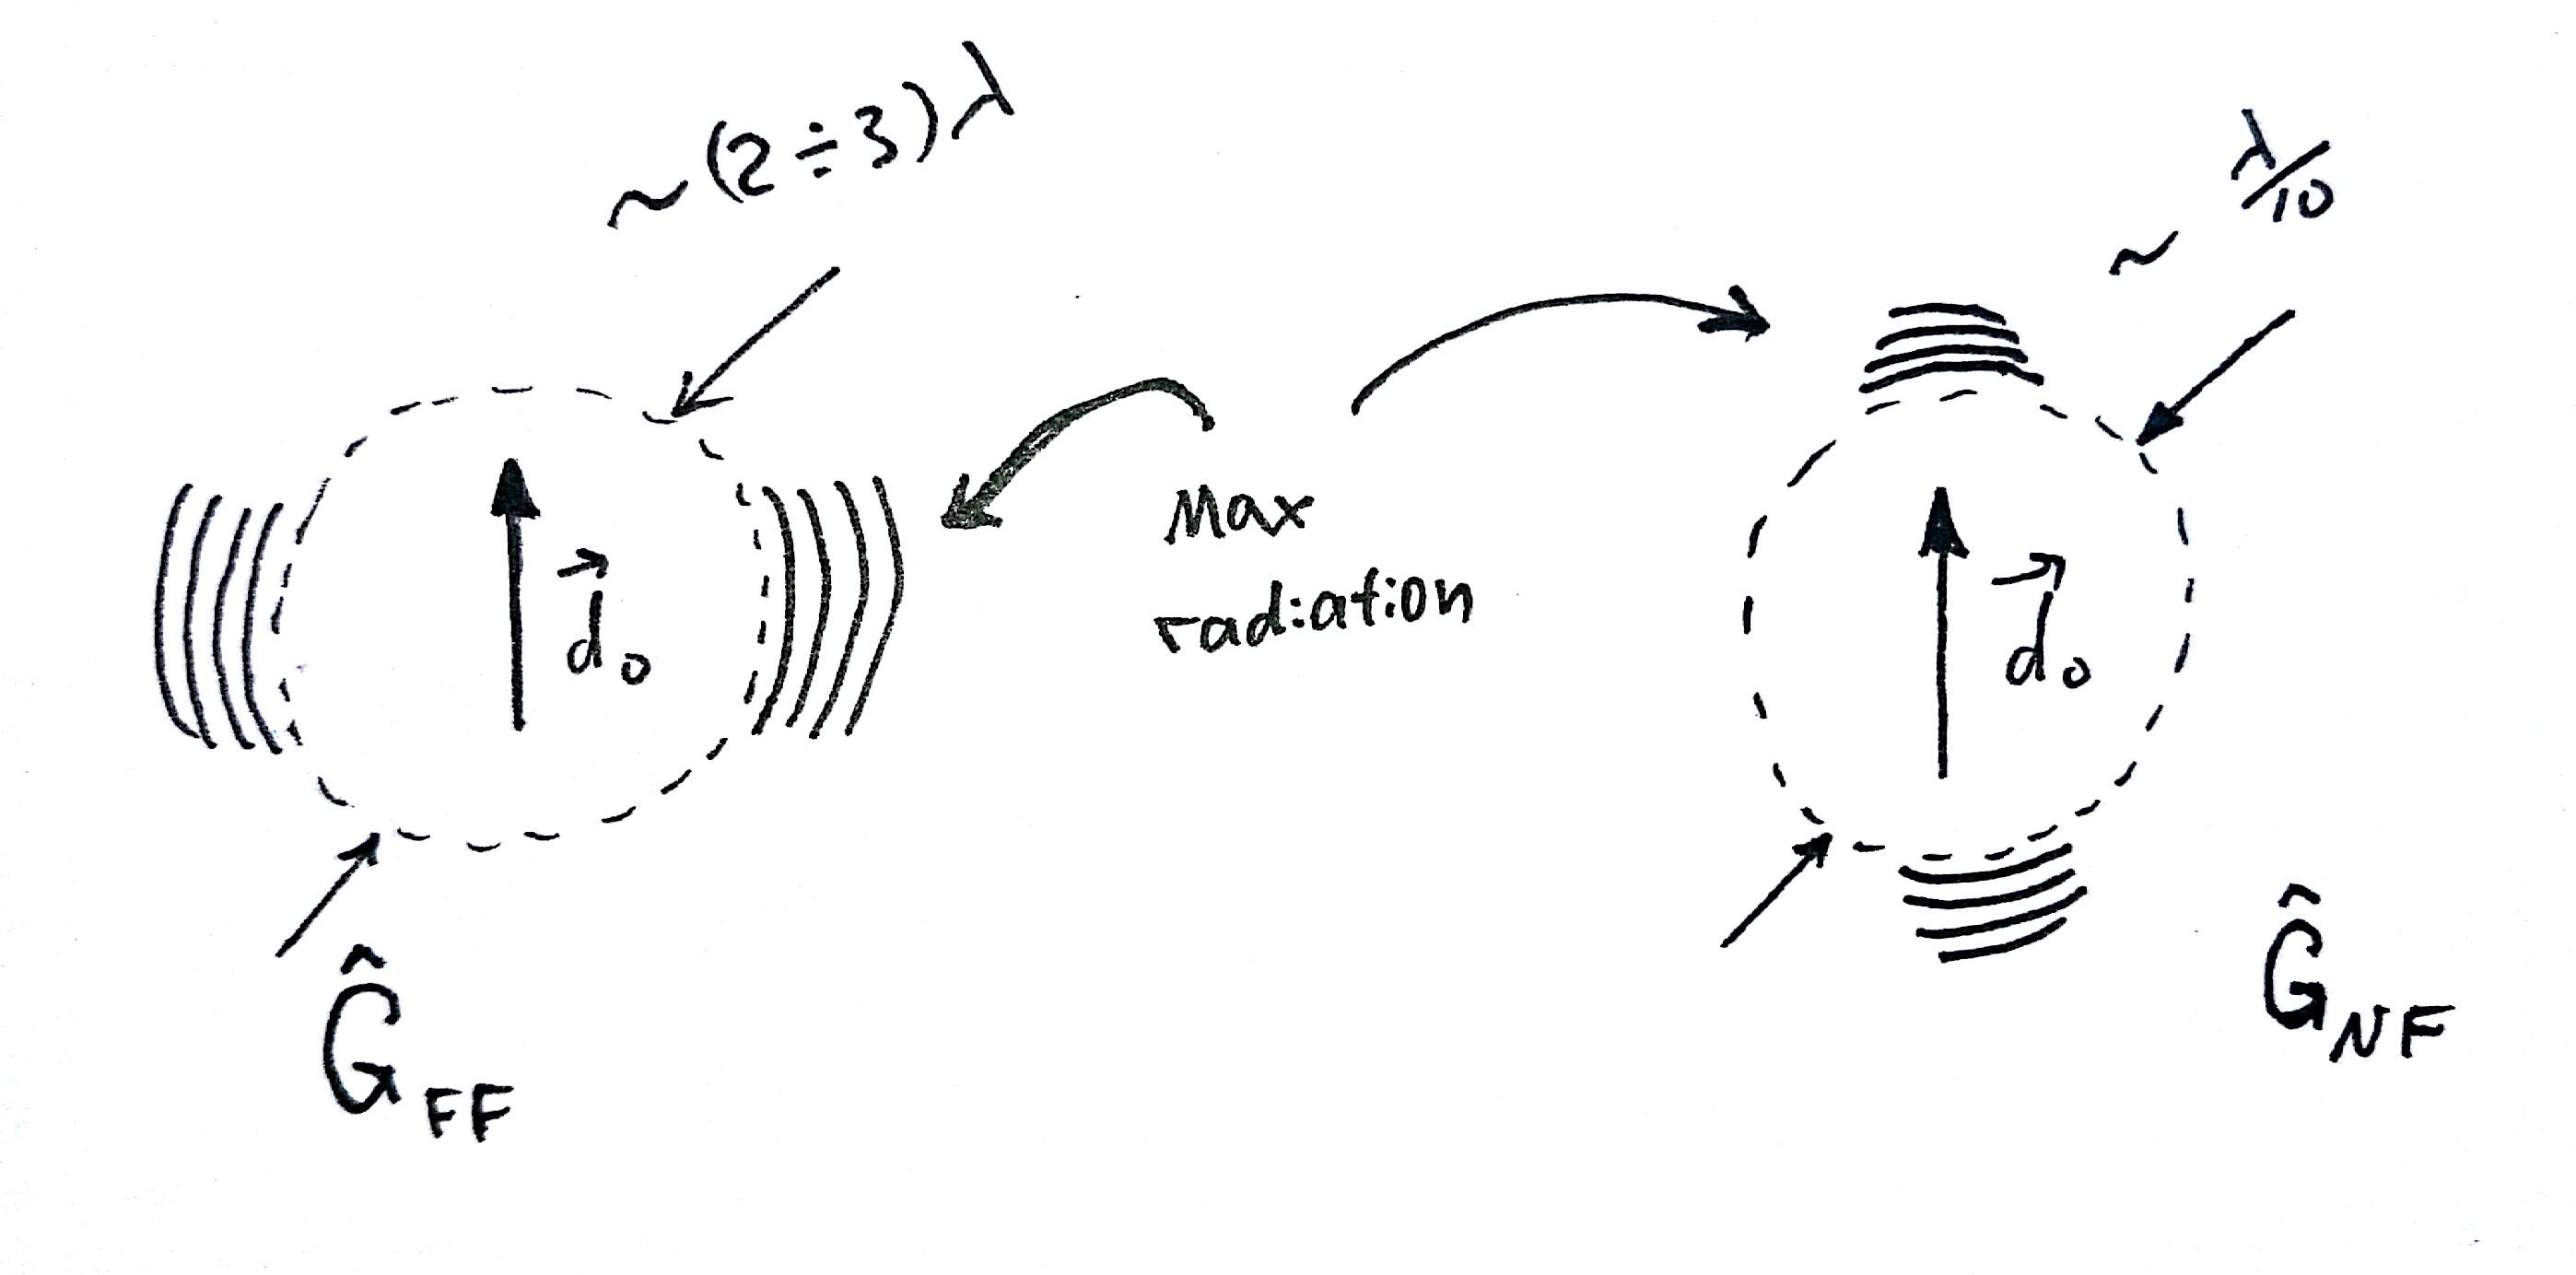
\includegraphics[width=0.6\linewidth]{fig/L8/radiation_1}
	\caption{Intuitive picture of positioning of maximum radiation of a dipole}
	\label{fig:radiation1}
\end{figure}


\subsection{Spontaneous relaxation and local density-of-state}

